\documentclass[12pt]{article}

%paquetes del idioma y codificacion
\usepackage[spanish]{babel}
\usepackage[utf8]{inputenc}
\usepackage[T1]{fontenc}
\usepackage{bookman}

%el indice
\usepackage{makeidx}

%paquetes matematicos
\usepackage{amsmath, amsfonts, amssymb}

%dimensiones
\usepackage[left=2.5cm, right=2.5cm, top=3cm]{geometry}

%para escribir codigo
\usepackage{listings}

% para contraer referencias
\usepackage{cite}

%para las imagenes y mas...
\usepackage{graphicx}
\usepackage{subfig}
\graphicspath{ {imagenes/} }
\usepackage{float}


\title{Reporte de prácticas primer periodo}
\author{Ian Mendoza Jaimes}


\begin{document}


\maketitle

\newpage

\tableofcontents

\newpage

\section{Introducción}

\newpage

\section{Alfabetos}
Los alfabetos se definen como un conjunto finito, no vacío de símbolos. Comúnmente se denotan con la letra griega $\sum$. Al definir un alfabeto, podemos tener acceso a seleccionar un conjunto finito de estos símbolos, a esto se le llama cadena o string. \cite{automatas}

\subsection{Descripción del problema}
Se necesita realizar un programa, que dado un alfabeto binario $\sum = \lbrace 0, 1 \rbrace $ en este caso, sea  capaz  de calcular e imprimir en un archivo de texto todas las palabras que puedan ser formadas por un alfabeto binario, es decir, \[{\sum}^{*} = {\sum}^{0}\cup{\sum}^{1}\cup{\sum}^{2}\cup\cdots\] Sin embargo, tiene limitaciones, pues es imposible calcular algo infinito, el programa deberá imprimir todas las combinaciones de las palabras con la longitud: $0 \leq n \leq 1000$.

\subsection{Código fuente}
El programa para este problema fue escrito en el lenguaje C. Esto debido a su alta velocidad de procesamiento, la cual es bastante necesaria si la longitud de las palabras es grande. El código utilizado para la resolución del problema se muestra a continuación:\\

Archivo: main.c
\lstset{language=C, breaklines=true, basicstyle=\footnotesize}
\begin{lstlisting}[frame=single]
#include "alfabeto.h"

int main(int argc, char const *argv[]) {
    char seleccion = '1';
    int continuar = 1;
    int continuar_modalidad = 1;
    int n = 0;
    char seleccion_tiro = ' ';

    srand(time(NULL));

    while(continuar == 1){
        printf("%s\n", "Seleccione la modalidad: \n1.- Automatico \n2.- Manual \n3.- Salir");
        scanf(" %c", &seleccion);

        if(seleccion == '1' || seleccion == '2'){
            continuar_modalidad = 1;
            while (continuar_modalidad == 1) {
                if(seleccion == '1'){
                    n = 1  + (rand()%5);
                }
                else{
                    printf("%s ", "Ingrese un n: ");
                    scanf("%d", &n);
                }

                iniciar_programa(n);

                if(seleccion == '2'){
                    printf("%s\n", "Desea ingresar otra n?: s/n");
                    scanf(" %c", &seleccion_tiro);
                    if(seleccion_tiro == 's' || seleccion_tiro == 'S'){
                        continuar_modalidad = 1;
                    }
                    else{
                        continuar_modalidad = 0;
                    }
                }
                else{
                    continuar_modalidad = rand()%2;
                    printf("%d\n", continuar_modalidad);
                }
            }
        }
        else{
            return 1;
        }
    }


    return 0;
}
}
\end{lstlisting}

\vspace{1em}
Archivo: alfabeto.c
\lstset{language=C, breaklines=true, basicstyle=\footnotesize}
\begin{lstlisting}[frame=single]
#include "alfabeto.h"

int iniciar_programa(int n){
  int tamanio_alfabeto = 2;
  char * alfabeto = NULL;
  alfabeto = (char *)malloc(tamanio_alfabeto * sizeof(char));
  iniciar_alfabeto(&alfabeto, tamanio_alfabeto);

  obtener_cadenas(alfabeto, tamanio_alfabeto, n);

  return 1;
}


int obtener_cadenas(char *alfabeto, int tamanio, int n){
    int i;
    int j;
    int * cadena_temporal = NULL;
    int salir = 0;

    FILE *archivo = NULL;

    archivo = fopen("cadenas.txt", "w");
    if (archivo == NULL) {
		printf("%s\n", "Error al abrir el archivo");
		exit(0);
	}

    fputs(" = { ", archivo);

    for(i = 1; i <= n; i++){
        cadena_temporal = (int*)calloc(i, sizeof(int));
        while(salir == 0){
            escribir_palabra(archivo, cadena_temporal, alfabeto, i);
            for(j = i -1; j > -1; j--){
                *(cadena_temporal + j) = *(cadena_temporal + j) + 1;
                if( *(cadena_temporal + j) > (tamanio -1)){
                    *(cadena_temporal + j) = 0;
                }
                else{break;}
            }
            if(j == -1){
                free(cadena_temporal);
                break;
            }
        }
        printf("Va en n = %d\n", i);
    }
    fputs(" }", archivo);
    fclose(archivo);

    return 1;
}

int escribir_palabra(FILE *archivo, int * cadena_temporal, char * alfabeto, int tamanio){
    int i;
    fputs(", ", archivo);
    for(i = 0; i < tamanio; i++){
        fputc(*(alfabeto + *(cadena_temporal + i)) , archivo);
    }
    return 1;
}

int iniciar_alfabeto(char **alfabeto, int tamanio){
    int i;
    for(i = 0; i < tamanio; i++){
        *(*alfabeto + i) = i + '0';
    }
    return  1;
}
\end{lstlisting}

\vspace{1em}
Archivo: alfabeto.h
\lstset{language=C, breaklines=true, basicstyle=\footnotesize}
\begin{lstlisting}[frame=single]
#ifndef __ALFABETO_H__
#define __ALFABETO_H__

#include <stdio.h>
#include <string.h>
#include <stdlib.h>
#include <time.h>


int iniciar_programa();
int iniciar_alfabeto(char **, int);
int escribir_palabra(FILE *, int *,char*, int);
int obtener_cadenas(char *, int, int);

#endif
\end{lstlisting}

\newpage
\subsection{Pruebas}
En cuanto a las pruebas, a continuación se mostraran una serie de imágenes capturadas al momento de ejecutar el programa. Los resultados arrojados por el programa anterior son:\\

Para la selección en modo automático:

\begin{figure}[H]
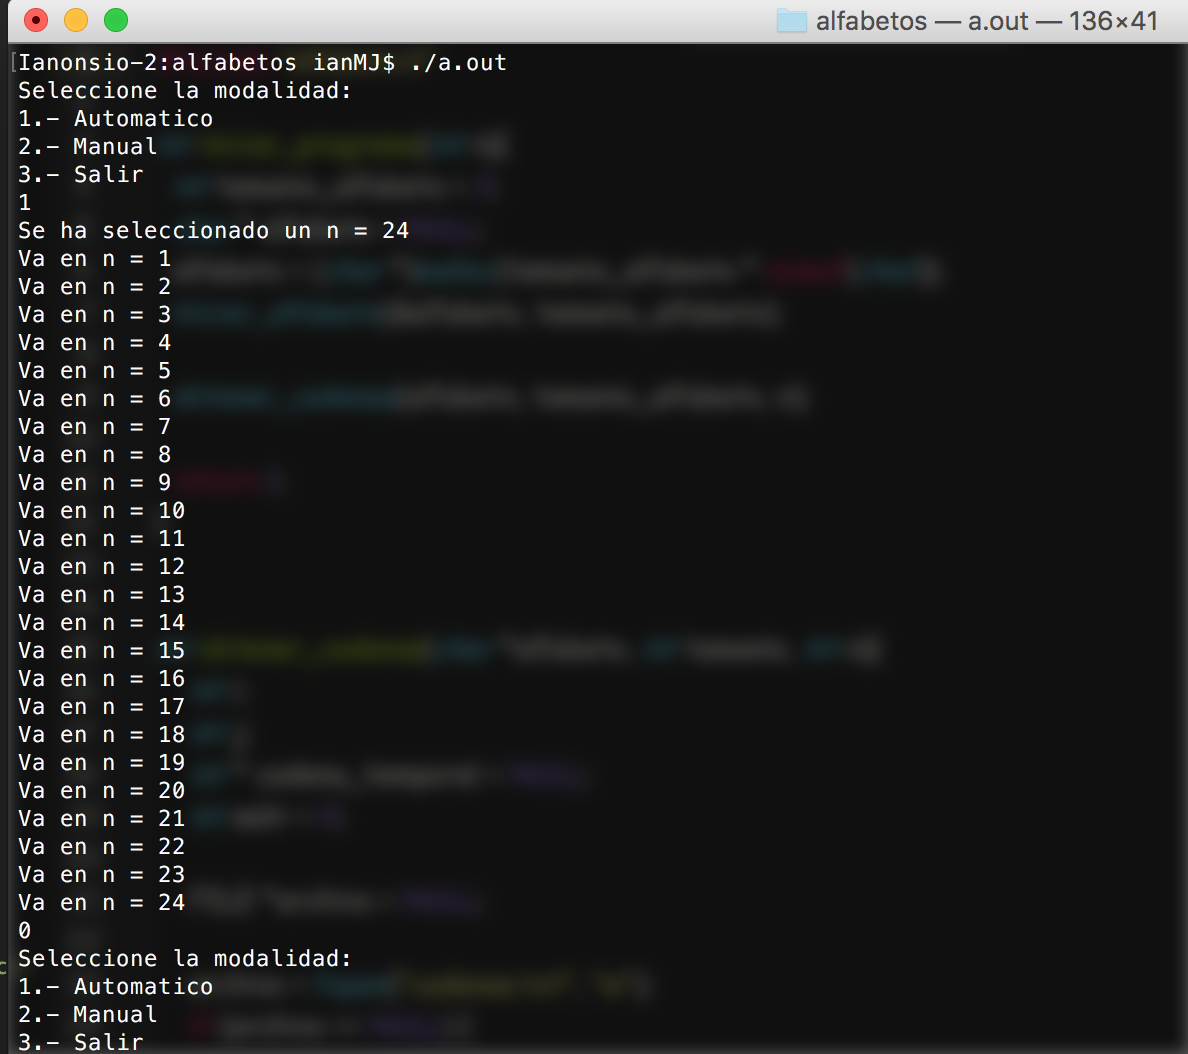
\includegraphics[width=\textwidth, height=7cm]{alfabetos_automatico}
\label{fig:auto_alfabeto}
\caption{Selección de un n = 24 de forma automática}
\end{figure}

\vspace{1em}

\begin{figure}[H]
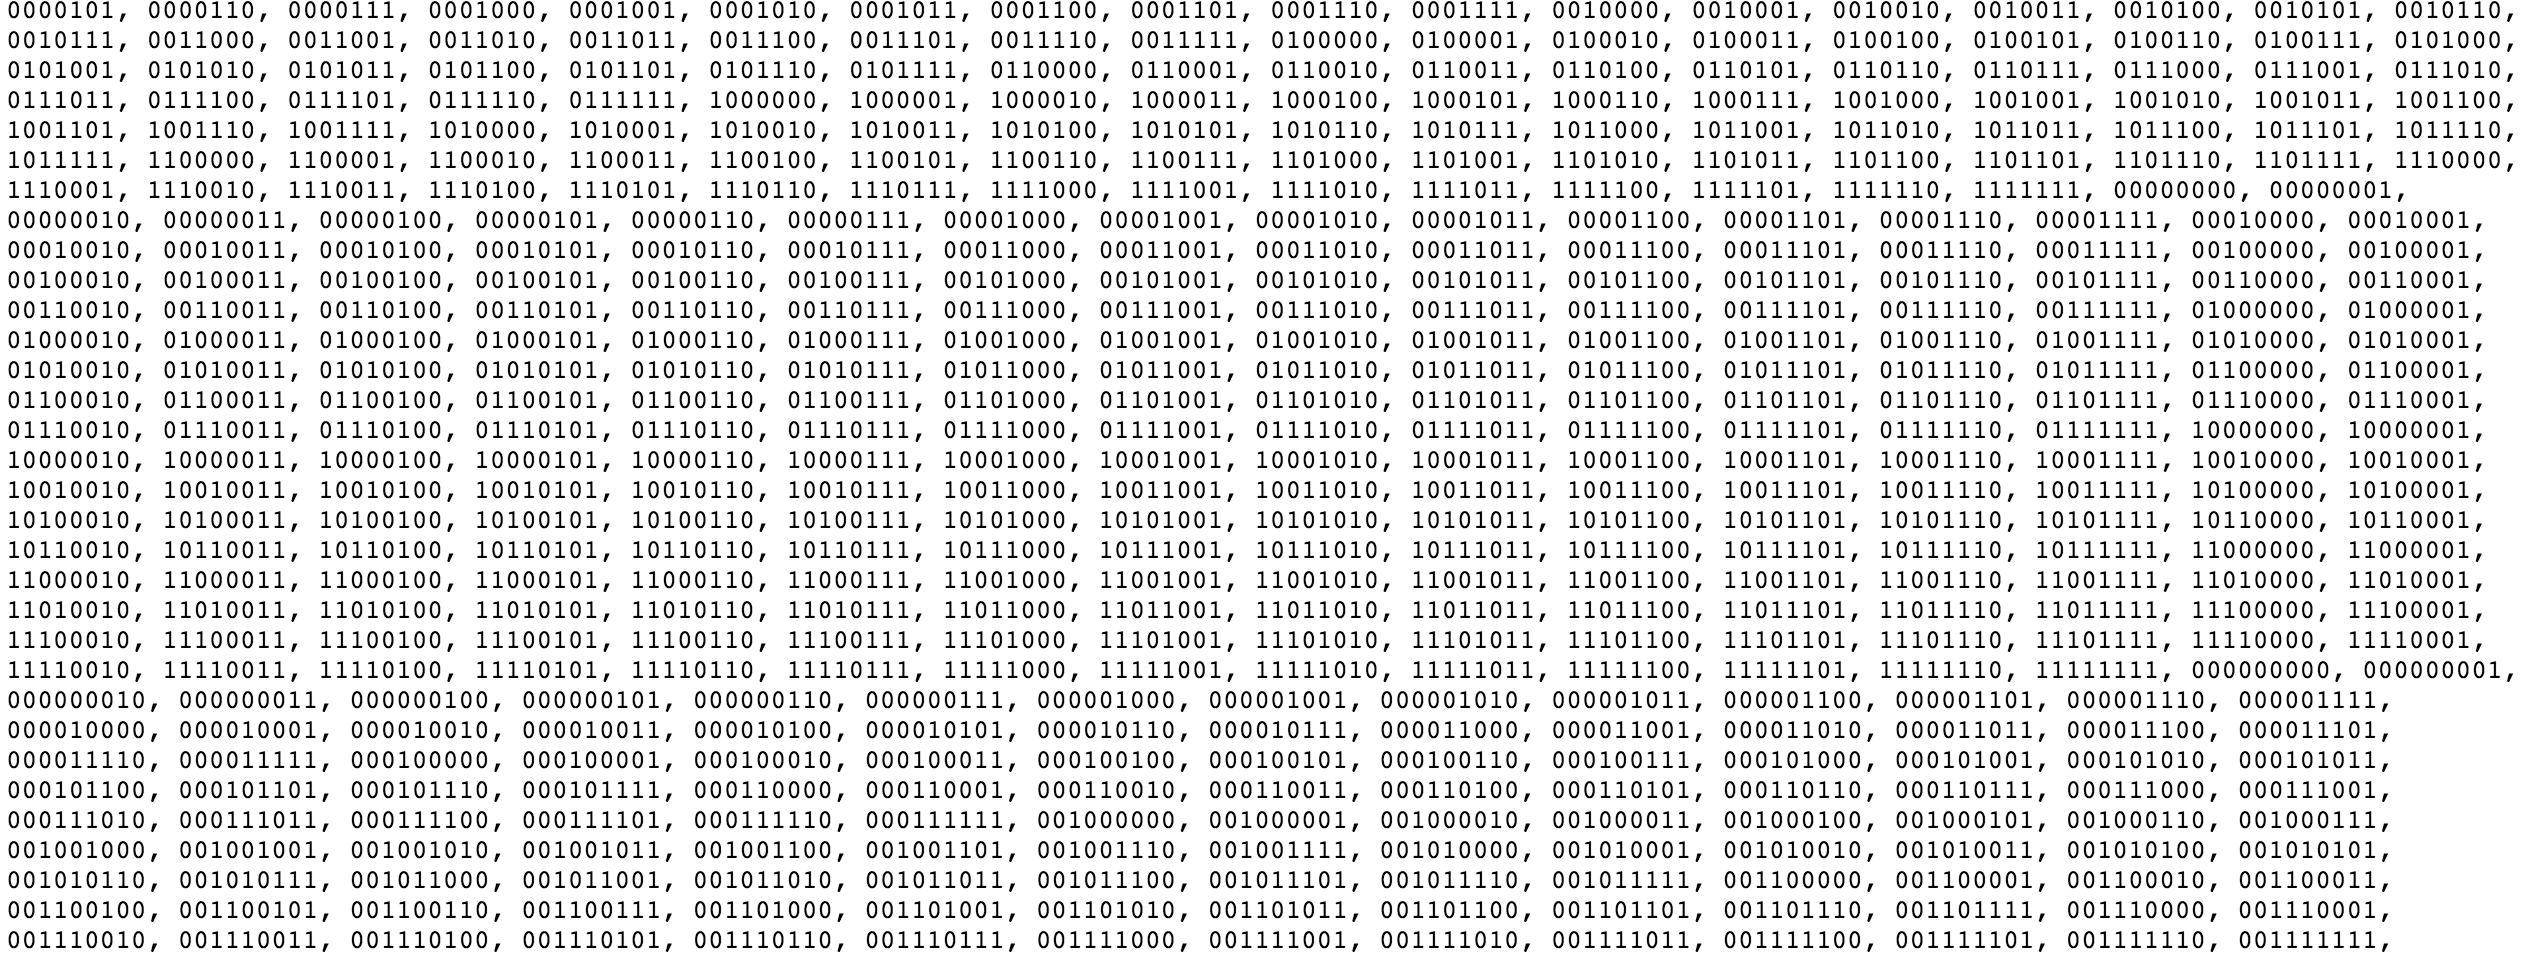
\includegraphics[width=\textwidth, height=6cm]{alfabeto_muestra}
\label{fig:auto_alfabeto_texto}
\caption{Texto producido por un n = 24}
\end{figure}

\vspace{1em}

Para la selección en modo manual:

\begin{figure}[H]
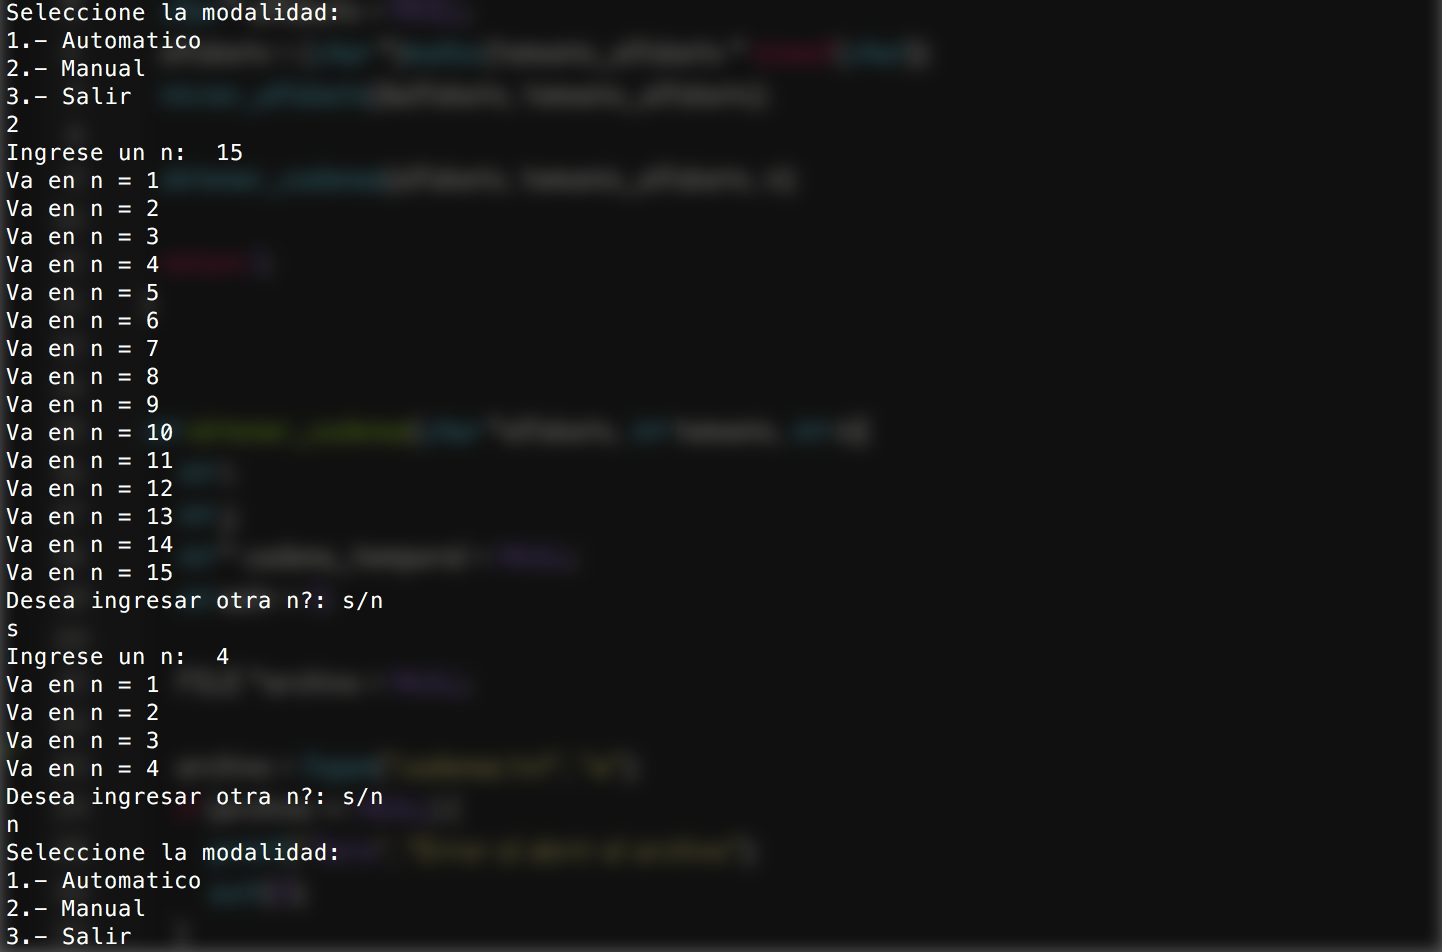
\includegraphics[width=\textwidth, height=7cm]{alfabetos_manual}
\label{fig:manual_alfabeto}
\caption{El resultado de escoger manualmente a n}
\end{figure}


\newpage
\section{Números primos}
Un número primo es aquel que solo puede ser divido entre si mismo o la unidad. A lo largo de la historia mucha gente los a estudiado y han propuesto numerosas maneras de encontrarlos. Algunos ejemplos de ello son la criba de Eratóstenes o la criba de Euler. En esta sección presentaremos un programa capaz de calcular todos los números primos en un intervalo dado.

\subsection{Descripción del problema}
Realizar un programa capaz de encontrar todos los números primos dentro de un intervalo dado por: $0 \leq n \leq 1000$. Además, deberá convertir dichos números de su representación decimal a su representación binaria y guardarlos en un archivo de texto. Después, se debe proceder a graficar la cantidad de ceros y unos que aparecen dependiendo de n.

\subsection{Código}
El programa, en este caso, fue escrito en Python. Fue seleccionado este lenguaje por la facilidad que presenta al manejar estructuras de datos como listas, pilas, etc. A continuación se presenta el código utilizado:\\


Archivo: main.py
\lstset{language=Python, breaklines=true, basicstyle=\footnotesize}
\begin{lstlisting}[frame = single]
from metodos import *
from random import random

def main():
    archivo = open("primos.txt", "w")
    archivo.write("")
    archivo.close()
    seguir = True
    while seguir:
        print("\n\nSelecciona el modo en que se ejecutara el programa: \n 1.- Automatico \n 2.- Manual \n 3.- Salir")
        try:
            seleccion = int(input())
            if seleccion > 0 and seleccion <= 2:
                iniciar_programa(seleccion)
            elif seleccion == 3:
                return 1;
            else:
                raise Exception()
        except Exception as e:
            print("Por favor ingrese un dato valido.")


def iniciar_programa(seleccion=1):
    numeros_primos = []
    numeros_primos_binarios = []
    numero_ceros_unos = []
    n = 0
    continuar = True
    archivo = None

    while continuar:
        if seleccion == 2:
            n = ingresar_datos("\nIngrese un numero limite ( 0 < n <= 1000): ")
        else:
            n = int(random() * 1000)
            print("\nFue seleccionado un n = ", n)
            
        archivo = open("primos.txt", "a")

        numeros_primos = encontrar_primos(numeros_primos, n)
        numeros_primos_binarios = convertir_primos_a_binarios(numeros_primos, archivo)
        numero_ceros_unos = contar_ceros_unos(numeros_primos_binarios)

        imprimir_ceros_unos(numero_ceros_unos, numeros_primos)
        
        archivo.close()

        if seleccion == 1:
            continuar = int(random() * 100) % 2
        else:
            eleccion = ingresar_datos("\nDesea ingresar otra n?  \n1.- Si \n2.- No \n")
            if eleccion != 1:
                continuar = False
                


def ingresar_datos(texto):
    while True:
        try:
            dato_n = int(input(texto))
            if dato_n > 0 and dato_n <= 1000:
                return dato_n
            else:
                raise Exception()
        except Exception as e:
            print("Por favor ingrese un dato valido")


def imprimir_ceros_unos(numero_ceros_unos, numeros_primos):
    contador = 0
    print (numeros_primos)
    print("{ numero primo, numero de unos }")
    while contador < len(numeros_primos):
        print("{",numeros_primos[contador], ",",numero_ceros_unos[contador][1],"}", end=", ")
        contador += 1

main()
\end{lstlisting}

\vspace{1em}

Archivo: metodos.py
\lstset{language=Python, breaklines=true, basicstyle=\footnotesize}
\begin{lstlisting}[frame=single]
def encontrar_primos(numeros_primos, n):
    if n == 1:
        return numeros_primos

    if len(numeros_primos) == 0:
        numeros_primos.append(2)

    for x in range(2,n+1):
        es_primo = True

        for y in numeros_primos:
            if x%y == 0:
                es_primo = False
                break

        if es_primo:
            numeros_primos.append(x)

    return numeros_primos


def convertir_primos_a_binarios(numeros_primos, archivo):
    numeros_primos_binarios = []
    for x in numeros_primos:
        numeros_primos_binarios.append(bin(x)[2:])
        archivo.write(", " + bin(x)[2:])

    return numeros_primos_binarios


def contar_ceros_unos(numeros_primos_binarios):
    numero_ceros_unos = []
    contador_ceros = 0
    contador_unos = 0
    for x in numeros_primos_binarios:
        contador_unos = 0
        contador_ceros = 0
        for y in x:
            if y == '0':
                contador_ceros += 1
            else:
                contador_unos += 1

        numero_ceros_unos.append([contador_ceros, contador_unos])

    return numero_ceros_unos

\end{lstlisting}

\subsection{Pruebas}
A continuación, se mostraran las imágenes de los resultados de ejecutar el programa en consola.\\

Para la selección de modo automático:
\begin{figure}[H]
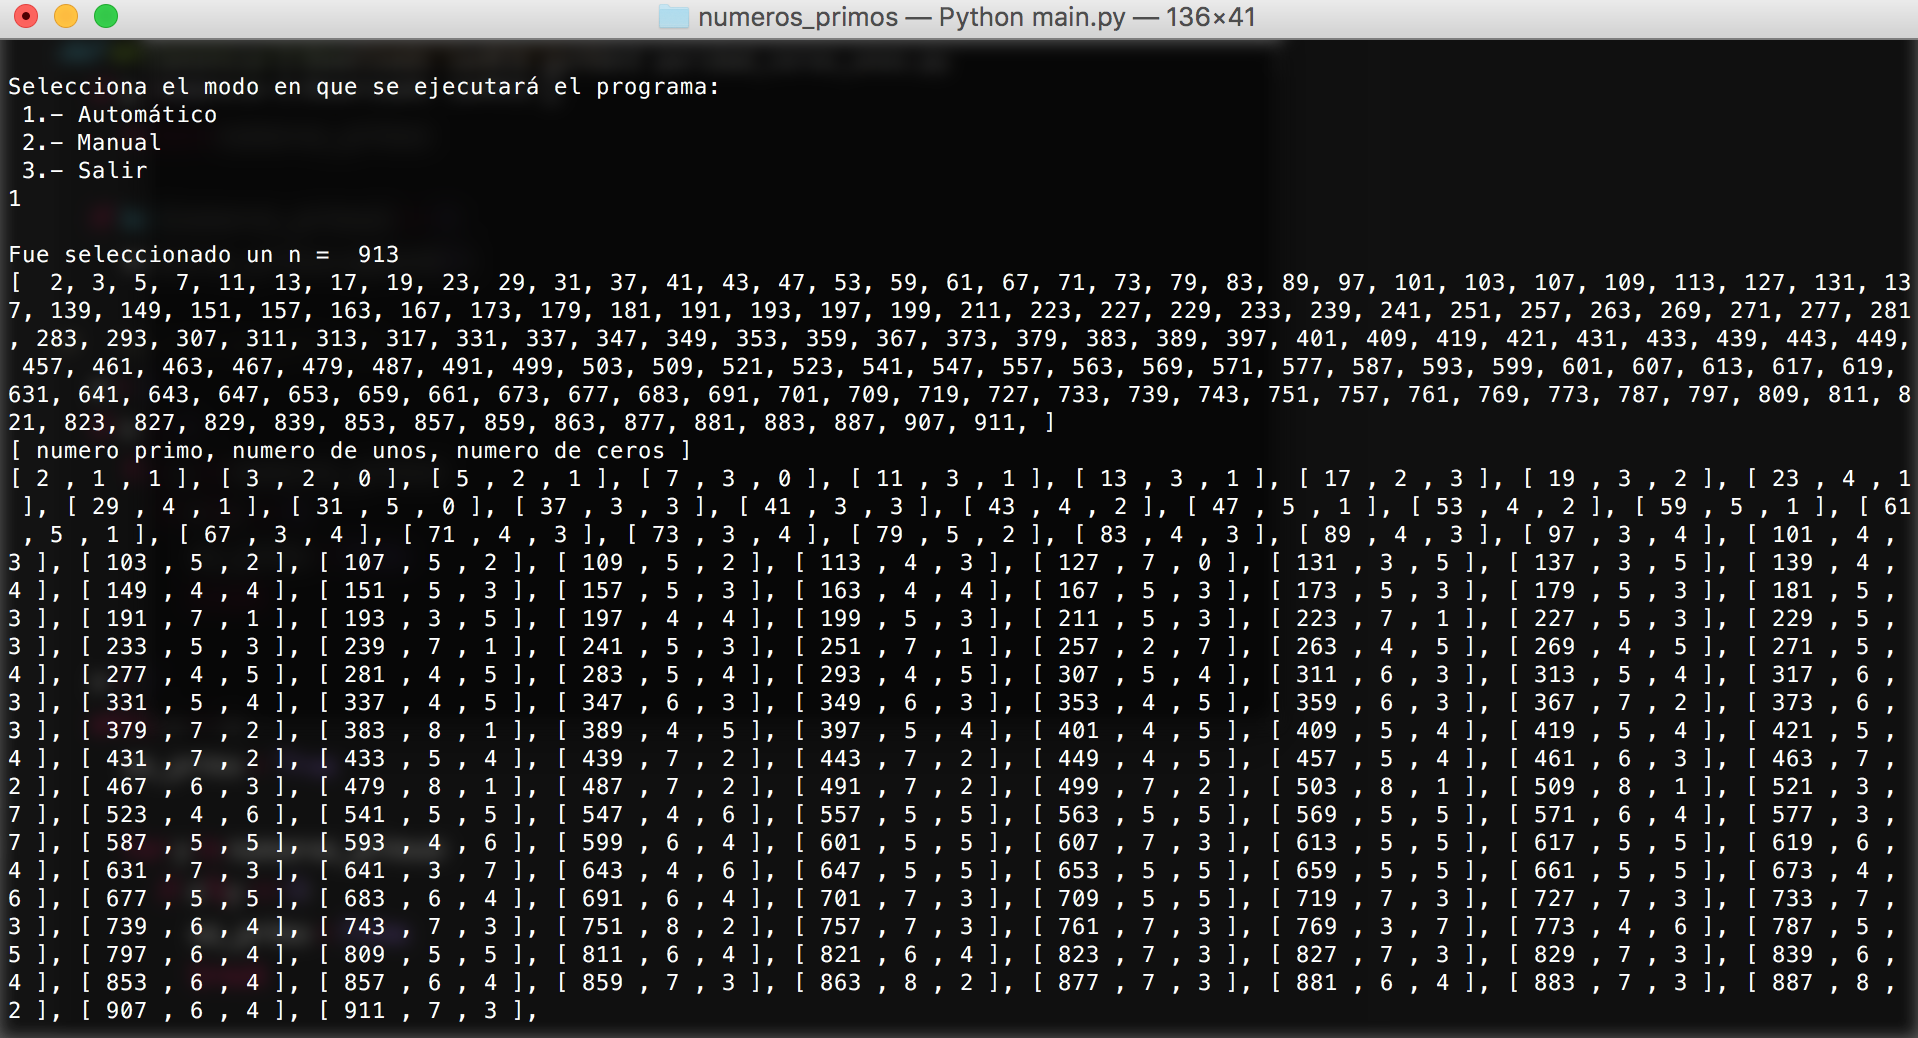
\includegraphics[width=\textwidth, height=13cm]{primos_automatico}
\caption{El resultado de seleccionar la modalidad automática}
\label{fig:primos_automatico}
\end{figure}

\vspace{1em}

Para la selección manual:
\begin{figure}[H]
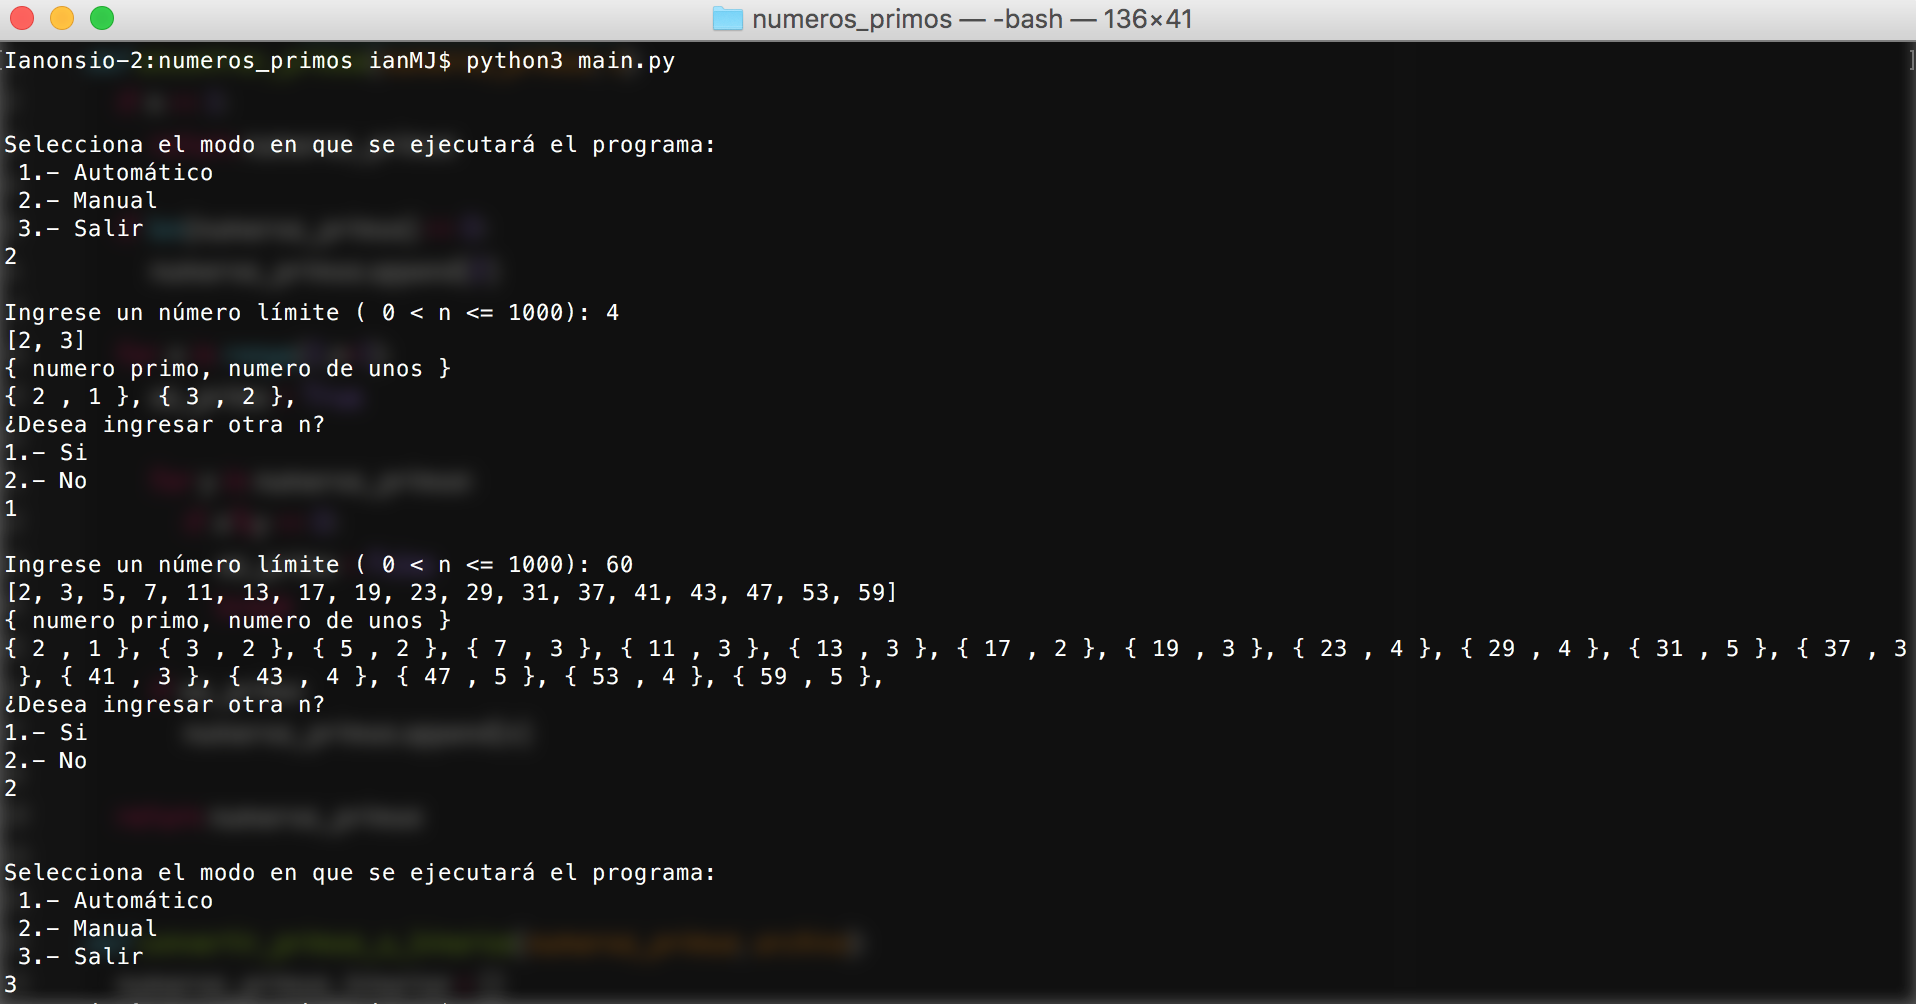
\includegraphics[width=\textwidth, height=10cm]{primos_manual}
\caption{El resultado de seleccionar la modalidad manual}
\label{fig:primos_manual}
\end{figure}


\newpage
\section{Palabras que terminan en ere}
Los autómatas son una forma de evaluar cadenas a través de una serie de estados. En concreto los autómatas determinísticos utilizan estados que solo pueden ser seguidos por otro estado. En esta sección se plantea un problema en el cual es muy conveniente utilizar un autómata para resolverlo y sirve como una introducción a esta teoría tan amplia.

\subsection{Descripción del problema}
Se tiene que elaborar un programa que pueda evaluar un texto y determinar cuales son las palabras que terminan con \textit{ere}. Además, deberá decir en que linea se encuentran. Para la realizacion de este programa, se debe de utilizar un autómata finito determinístico.


\subsection{Código}
El modelo del automata utilizado para resolver este programa es el siguiente:

\begin{figure}[H]
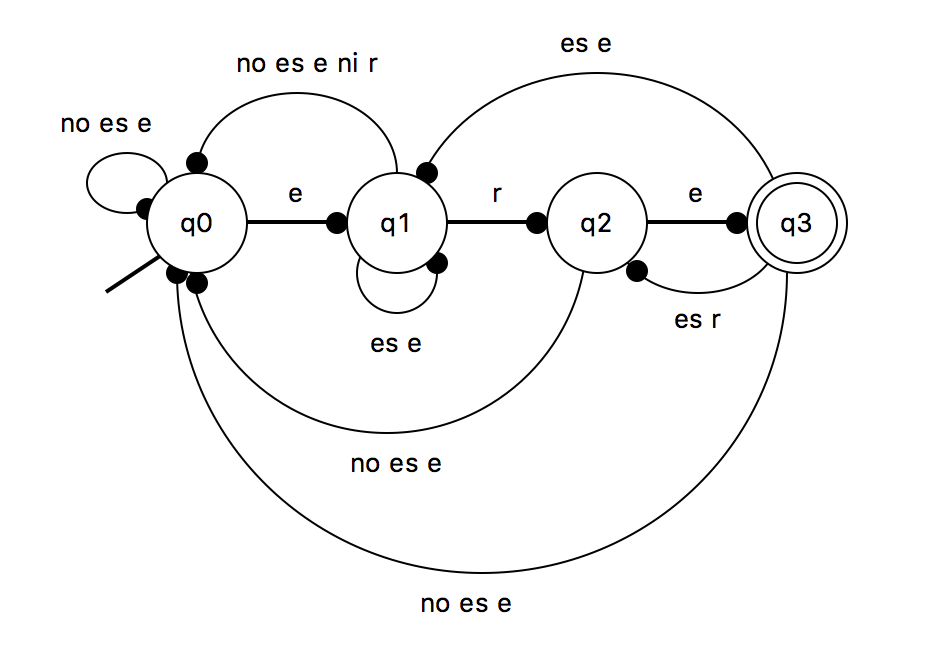
\includegraphics[width=\textwidth, height=10cm]{automata_ere}
\caption{El autómata utilizado para este problema}
\label{fig:automata_ere_modelo}
\end{figure}

El lenguaje utilizado para este programa fue Python en su versión 3.5. El código para resolver el problema es el siguiente:\\

Archivo: main.py
\lstset{language=Python, breaklines=true, basicstyle=\footnotesize}
\begin{lstlisting}[frame=single]
from automata import obtener_palabras, graficar_automata
from ctypes import *

def main():
    while seguir:
        try:
            palabras_aceptadas = []
            texto = ""
            archivo = None

            opcion = imprimir_menu()

            if opcion == 1:
                texto = input("\n\nIngrese un texto: \n")
                palabras_aceptadas = leer_texto(texto)
            elif opcion == 2:
                texto = input("\n\nIngrese el nombre de un archivo: \n")
                archivo = open(texto, "r")
                palabras_aceptadas = leer_archivo(archivo)
            elif opcion == 3:
                print("Sera utilizado el archivo heart.txt")
                archivo = open("heart.txt", "r")
                palabras_aceptadas = leer_archivo(archivo)
            elif opcion == 4:
                graficar_automata()
            else:
                return 0

            imprimir_palabras_aceptadas(palabras_aceptadas, opcion)

            texto = input("\n\nDesea ingresar otra cosa? [s/n]: ")
            if (texto != 's') and (texto != 'S'):
                seguir = False

        except Exception as e:
            print("Uuups!, parece que tuvimos un problema: ", e)
    return 1


def imprimir_menu():
    seguir = True
    while seguir:
        try:
            opcion = int(input("\n\nIngrese la opcion que desea: \n1.- Ingresar texto \n2.- Ingresar un archivo \n3.- Automatico \n4.- Ver grafico del automata \n5.- Salir\n"))
            return opcion
        except Exception as e:
            print("Por favor, ingrese un dato valido.")


def leer_texto(texto):
    texto += " "
    aceptadas = obtener_palabras(texto)
    return aceptadas


def leer_archivo(archivo):
    aceptadas = None
    palabras_aceptadas = []
    contador = 1
    for linea in archivo:
        aceptadas = obtener_palabras(linea)
        palabras_aceptadas.append([contador, aceptadas])
        contador += 1

    archivo.close()
    return palabras_aceptadas


def imprimir_palabras_aceptadas(palabras_aceptadas, seleccion):
    print("\n\n\n")
    if seleccion == 1:
        print("Palabras aceptadas: ", palabras_aceptadas)
    else:
        contador = 0
        for x in palabras_aceptadas:
            if len(x[1]) > 0:
                print("Linea ", x[0], " palabras aceptadas: ", x[1])


main()

\end{lstlisting}

\vspace{1em}

Archivo: automata.py
\lstset{language=Python, breaklines=true, basicstyle=\footnotesize}
\begin{lstlisting}[frame=single]
from tkinter import *
import time

def obtener_palabras(texto):
    estado = 0
    palabras_aceptadas = []
    temporal = ''
    letra_auxiliar = ''
    for x in texto:
        letra_auxiliar = x
        letra_auxiliar.lower()

        estado = automata(estado, letra_auxiliar)

        if estado == -1:
            estado = 0
            temporal = ''
        elif estado == 4:
            palabras_aceptadas.append(temporal)
            estado = 0
            temporal = ''
        else:
            temporal += x

    return palabras_aceptadas

def automata(estado, letra_auxiliar):
    alfabeto = [97, 122]
    if estado == 0:
        return estado_cero(alfabeto,letra_auxiliar)
    elif estado == 1:
        return estado_uno(alfabeto,letra_auxiliar)
    elif estado == 2:
        return estado_dos(alfabeto,letra_auxiliar)
    elif estado == 3:
        return estado_tres(alfabeto,letra_auxiliar)
    else:
        return -1


def estado_cero(alfabeto,letra):
    if(ord(letra) >= alfabeto[0] and ord(letra) <= alfabeto[1]):
        if letra == 'e':
            return 1
        else:
            return 0
    else:
        return -1


def estado_uno(alfabeto,letra):
    if(ord(letra) >= alfabeto[0] and ord(letra) <= alfabeto[1]):
        if letra == 'e':
            return 1
        elif letra == 'r':
            return 2
        else:
            return 0
    else:
        return -1


def estado_dos(alfabeto,letra):
    if(ord(letra) >= alfabeto[0] and ord(letra) <= alfabeto[1]):
        if letra == 'e':
            return 3
        else:
            return 0
    else:
        return -1


def estado_tres(alfabeto,letra):
    if(ord(letra) >= alfabeto[0] and ord(letra) <= alfabeto[1]):
        if letra == 'e':
            return 1
        else:
            return 0
    else:
        return 4

def graficar_automata():
    raiz = Tk()
    raiz.title('Automata')
    raiz.geometry('500x350')
    canvas = Canvas(raiz, width=600, height=410, bg='white')
    canvas.place(x=0,y=0)
    canvas.pack(expand=YES, fill=BOTH)

    x = 90
    y = 100
    r = 50
    numero_circulos = 4
    opciones = ['e','r','e']
    canvas.create_line(x-20, y+r*1.2, x+.2*r, y+.8*r, width=2, fill='black')
    for i in range(numero_circulos):
        dibujos_especificos(canvas, i, x, y)
        x += r+50

    x = 90
    for i in range(numero_circulos):
        canvas.create_oval(x, y, x+r, y+r, width=1, fill='white')
        widget = Label(canvas, text='q'+str(i), fg='black', bg='white')
        widget.pack()
        canvas.create_window(x+.5*r, y+.5*r, window=widget)

        if i < numero_circulos-1:
            canvas.create_line(x+r, y+(r/2), x+r+50, y+(r/2), width=2, fill='black')
            widget = Label(canvas, text=opciones[i], fg='black', bg='white')
            widget.pack()
            canvas.create_window(x+r+25, y+(r/2)-15, window=widget)
            canvas.create_oval(x+r+40, y+(r/2)-5, x+r+50, y+(r/2)+5, width=1, fill='black')

        if i == numero_circulos -1:
            canvas.create_oval(x+5, y+5, x+r-5, y+r-5, width=1, fill='white')
        x += r+50

    raiz.mainloop()

def dibujos_especificos(canvas, i, x, y):
    if i == 0:
        xy = x+10, y-20, x+30, y+10
        canvas.create_oval(x-30,y-10, x+10,y+20, width=1)
        canvas.create_oval(x-5, y+13, x+5, y+23, width=1, fill='black')
        widget = Label(canvas, text='no es e', fg='black', bg='white')
        widget.pack()
        canvas.create_window(x-20, y-25, window=widget)
    elif i == 1:
        xy = x-75, y-40, x+25, y+40
        canvas.create_arc(xy, start=0, extent=180, style='arc')
        canvas.create_oval(x-80, y-10, x-70, y, width=1, fill='black')
        canvas.create_oval(x+5,y+30, x+45,y+70, width=1)
        widget = Label(canvas, text='no es e ni r', fg='black', bg='white')
        widget.pack()
        canvas.create_window(x-20, y-55, window=widget)
        canvas.create_oval(x+40,y+40, x+50,y+50, width=1, fill='black')
        widget = Label(canvas, text='es e', fg='black', bg='white')
        widget.pack()
        canvas.create_window(x+25, y+85, window=widget)
    elif i == 2:
        xy = x-180, y-70, x+20, y+130
        canvas.create_arc(xy, start=0, extent=-180, style='arc')
        widget = Label(canvas, text='no es e', fg='black', bg='white')
        widget.pack()
        canvas.create_window(x-75, y+145, window=widget)
        canvas.create_oval(x-180,y+50, x-170,y+60, width=1, fill='black')
    elif i == 3:
        xy = x-285, y-100, x+20, y+200
        canvas.create_arc(xy, start=0, extent=-180, style='arc')
        canvas.create_oval(x-290,y+45, x-280,y+55, width=1, fill='black')
        widget = Label(canvas, text='no es e', fg='black', bg='white')
        widget.pack()
        canvas.create_window(x-140, y+215, window=widget)
        xy = x-170, y+120, x+20, y-50
        canvas.create_arc(xy, start=0, extent=180, style='arc')
        canvas.create_oval(x-165,y+5, x-155,y-5, width=1, fill='black')
        widget = Label(canvas, text='es e', fg='black', bg='white')
        widget.pack()
        canvas.create_window(x-80, y-65, window=widget)

\end{lstlisting}

\subsection{Pruebas}
Los siguientes, son los resultados que se obtuvieron del programa anterior.

\begin{figure}[H]
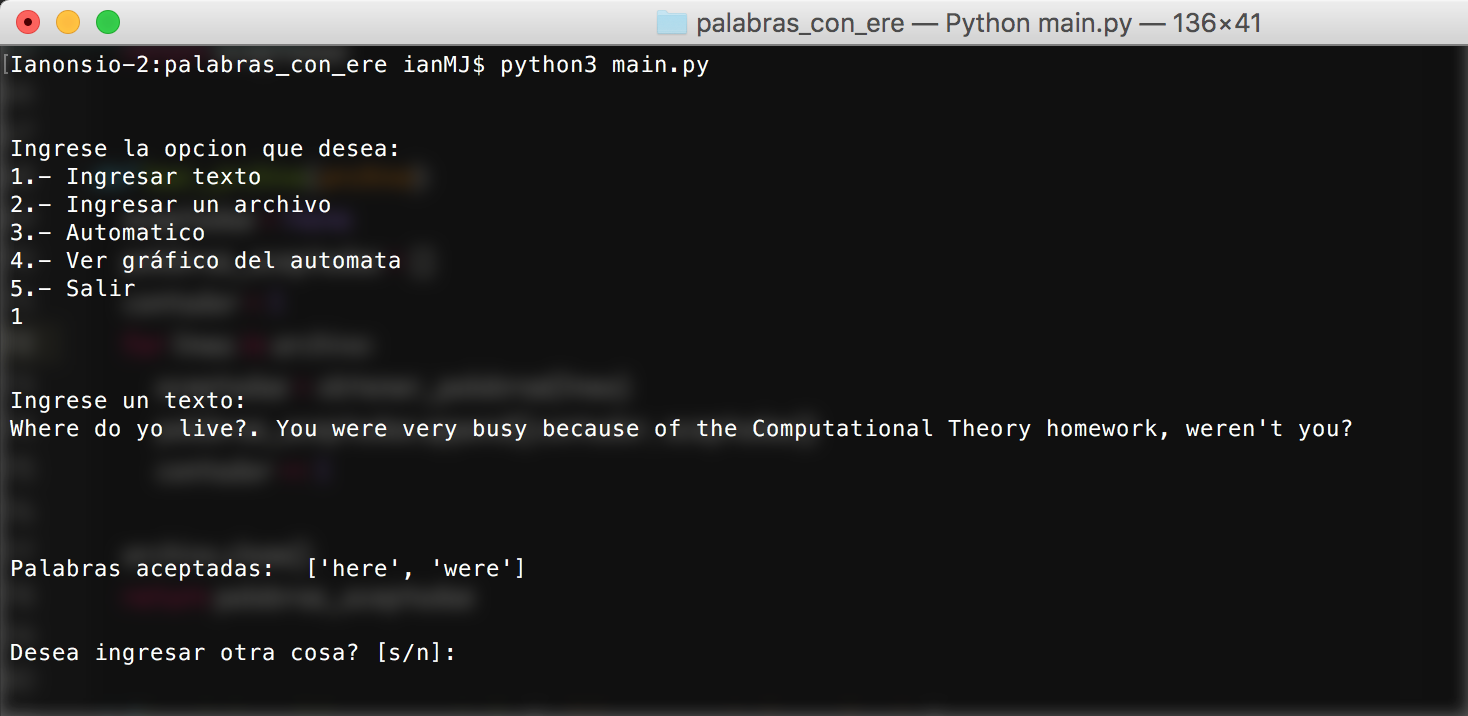
\includegraphics[width=\textwidth, height=8cm]{palabras_ere_texto}
\caption{Un texto analizado por el programa.}
\label{fig:automata_ere_texto}
\end{figure}

\begin{figure}[H]
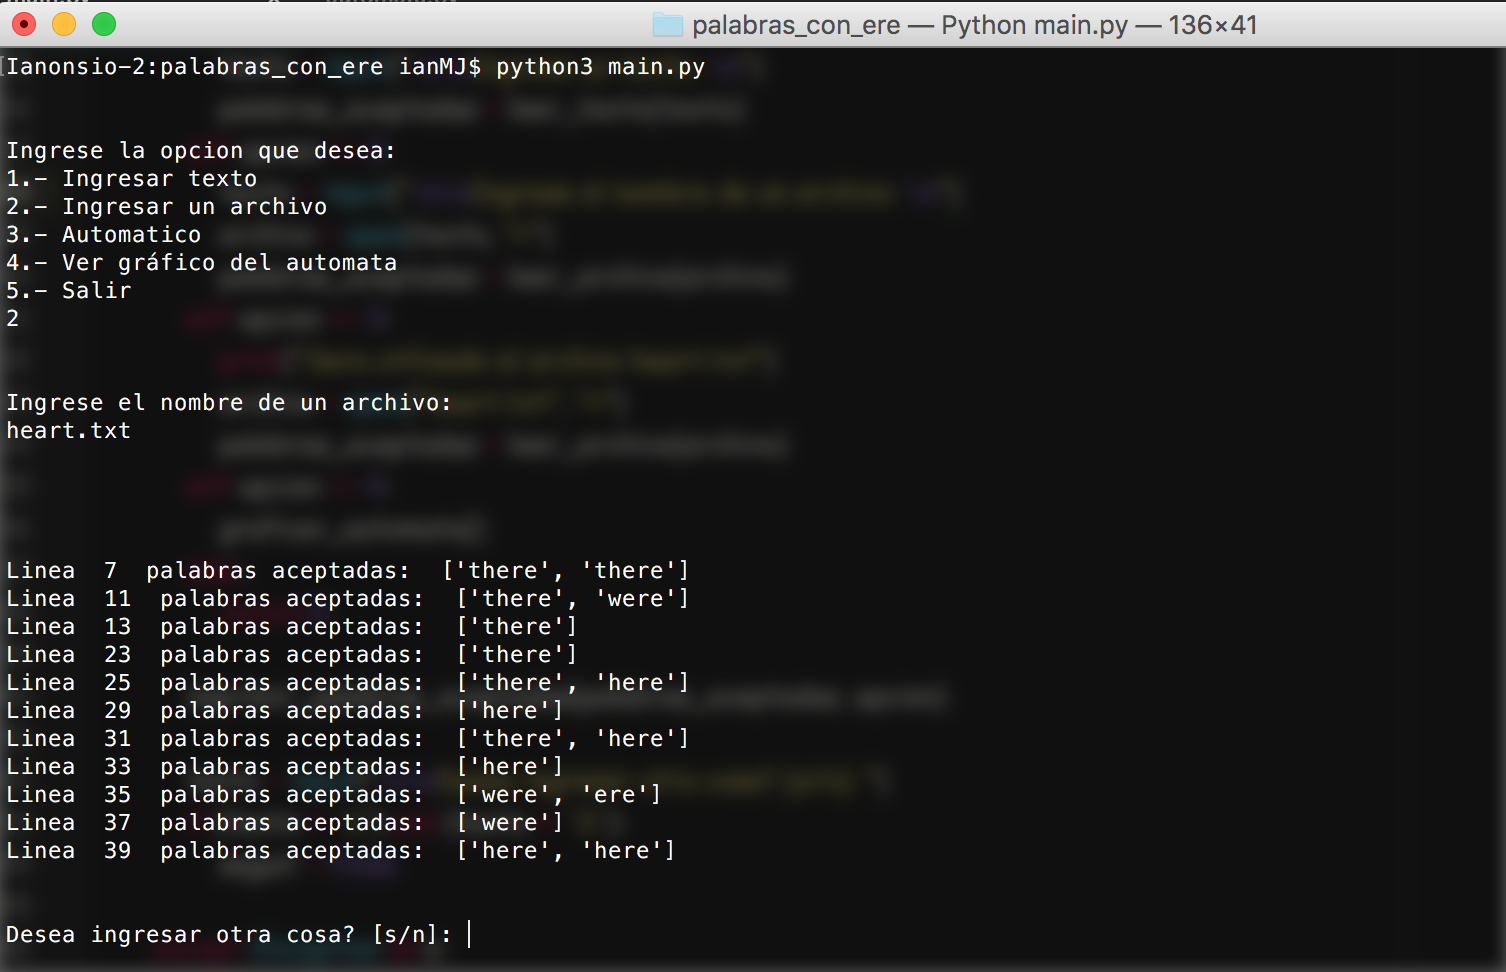
\includegraphics[width=\textwidth, height=8cm]{palabras_ere_archivo}
\caption{Un archivo analizado por el programa.}
\label{fig:automata_ere_archivo}
\end{figure}

\begin{figure}[H]
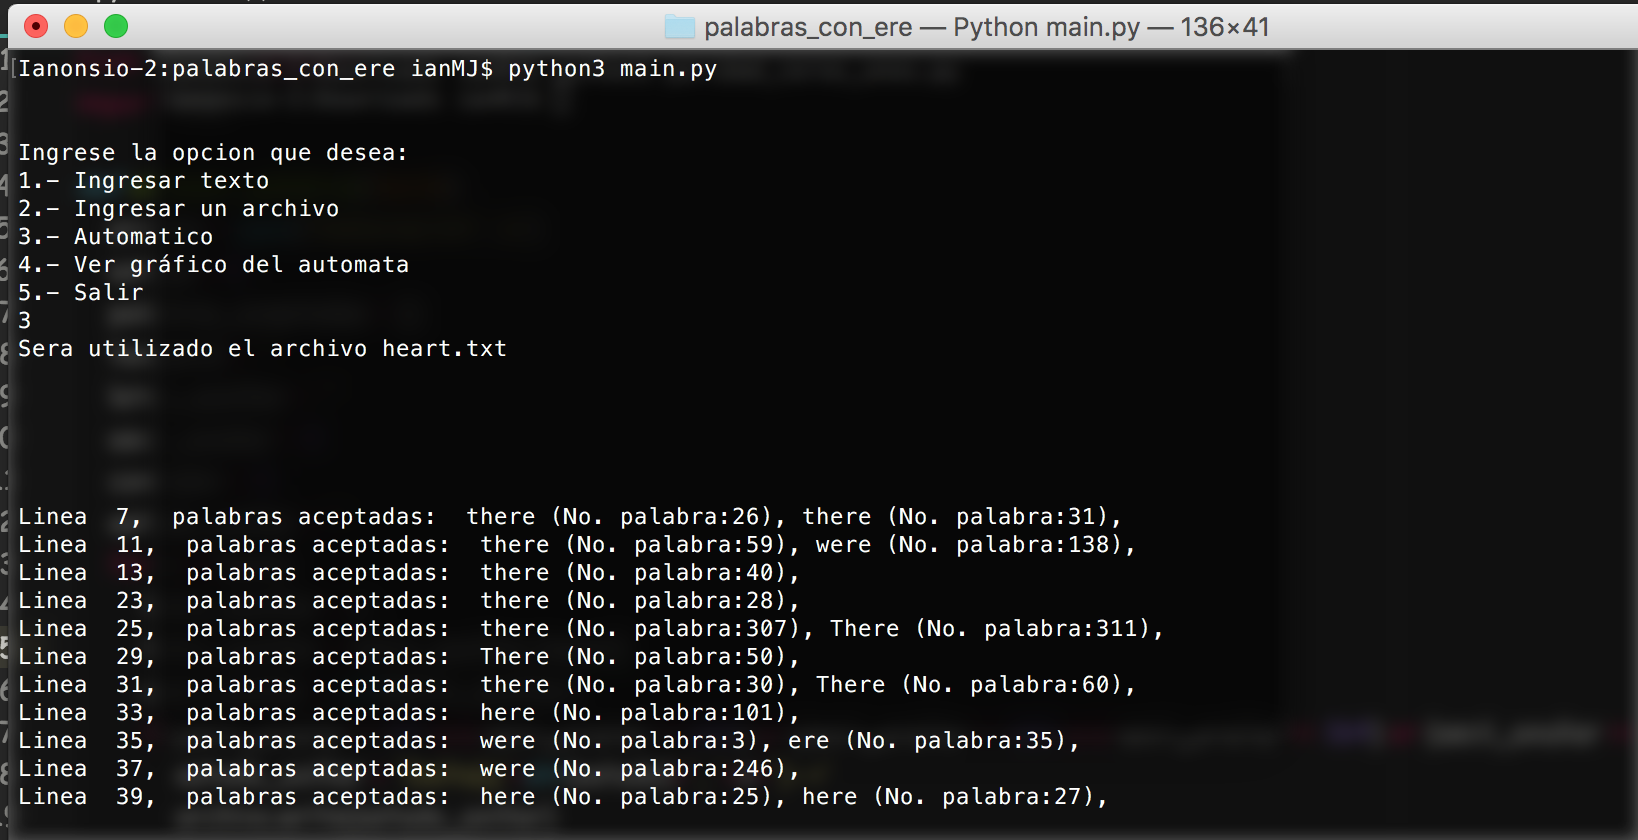
\includegraphics[width=\textwidth, height=8cm]{palabras_ere_auto}
\caption{Un archivo analizado de forma automática por el programa.}
\label{fig:automata_ere_auto}
\end{figure}

\newpage
\section{Paridad}

\newpage
\section{Protocolo}

\newpage
\section{Cadenas que terminan en 01}


\bibliographystyle{acm}
\bibliography{bibliografia}

\end{document}